\documentclass[11pt]{exam}
\usepackage{graphicx} % Required for inserting images
\usepackage{amssymb}
\usepackage{amsmath}
\usepackage{optidef}
\usepackage{listings}
\usepackage{xcolor} % for custom colors
\usepackage{minted} % for code

% === Make things tighter ===
\usepackage[margin=0.75in]{geometry} % <- widen/narrow by changing 1.25in
\usepackage{setspace}
% \setstretch{0.95} % line spacing
\usepackage{enumitem}
% \setlist{nosep}  % removes vertical space around lists
% \setlist[itemize]{topsep=3pt, itemsep=3pt, parsep=1pt, partopsep=0pt}
% \setlist[enumerate]{topsep=3pt, itemsep=3pt, parsep=1pt, partopsep=0pt}
\usepackage{titlesec}
% \titlespacing*{\section}{0pt}{4.0ex plus 0.5ex minus 0.5ex}{0.8ex}
% \titlespacing*{\subsection}{0pt}{3.0ex plus 0.3ex minus 0.3ex}{0.6ex}
% \titlespacing*{\subsubsection}{0pt}{2.0ex plus 0.2ex minus 0.2ex}{0.4ex}
% \titlespacing*{\paragraph}{0pt}{1.5ex plus 0.2ex minus 0.2ex}{0.4ex}


\lstset{
  language=Python,
  basicstyle=\ttfamily\small,
  keywordstyle=\color{blue},
  stringstyle=\color{red},
  commentstyle=\color{gray},
  showstringspaces=false,
  frame=single,
  breaklines=true
}
\title{15.081 Mathematical programming, HW5}
\author{Erich Trieschman}
\date{2025.11.20}
\begin{document}
\maketitle

\begin{questions}
    % ============ QUESTION 7.9 ==============
    \question \textbf{Exercise 7.9:} Given the uncapacitated network flow problem
    \begin{center}
        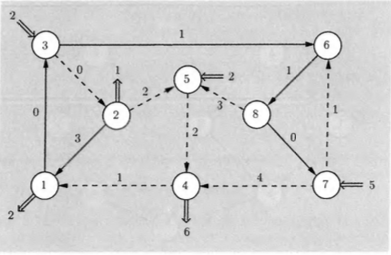
\includegraphics[width=0.5\textwidth]{hw5_exercise7.9.png}
    \end{center}
    \begin{parts}
        \part What is the matrix $A$ corresponding to this problem?
        \begin{align*}
            % 8x11 matrix of placeholders with row and column labels
            % Use array for labeled rows/columns
            \begin{array}{c|rrrrrrrrrrrr}
                & (1,3) & (2,1) & (2,5) & (3,2) & (3,6) & (4,1) & (5,4) & (6,8) & (7,4) & (7,6) & (8,5) & (8,7) \\
                \hline
                1 &  1  & -1 &  0 &  0 &  0 & -1 &  0 &  0 &  0 &  0 &  0 &  0 \\
                2 &  0  &  1 &  1 & -1 &  0 &  0 &  0 &  0 &  0 &  0 &  0 &  0 \\
                3 & -1  &  0 &  0 &  1 &  1 &  0 &  0 &  0 &  0 &  0 &  0 &  0 \\
                4 &  0  &  0 &  0 &  0 &  0 &  1 & -1 &  0 & -1 &  0 &  0 &  0 \\
                5 &  0  &  0 & -1 &  0 &  0 &  0 &  1 &  0 &  0 &  0 & -1 &  0 \\
                6 &  0  &  0 &  0 &  0 & -1 &  0 &  0 &  1 &  0 & -1 &  0 &  0 \\
                7 &  0  &  0 &  0 &  0 &  0 &  0 &  0 &  0 &  1 &  1 &  0 & -1 \\
                8 &  0  &  0 &  0 &  0 &  0 &  0 &  0 & -1 &  0 &  0 &  1 &  1 \\
            \end{array}
            % To add row and column labels in LaTeX, use the array environment and put labels in the first row (after &) and first column of each row.
        \end{align*}

        \part Solve the problem using the network simplex algorithm. Start with the tree indicated by the dashed arcs in the figure.
        \newline Begin by defining simplex problem constants
        \begin{align*}
            b^\top &= \begin{array}{|cccccccc|}
                1& 2& 3& 4& 5& 6& 7& 8\\\hline
                -2 & -1 & 2 & -6 & 2 & 0 & 5 & 0
            \end{array}\\
            c^\top &= \begin{array}{|cccccccccccc|}
                (1,3) & (2,1) & (2,5) & (3,2) & (3,6) & (4,1) & (5,4) & (6,8) & (7,4) & (7,6) & (8,5) & (8,7)\\
                \hline
                0 & 3 & 2 & 0 & 1 & 1 & 2 & 1 & 4 & 1 & 3 & 0
            \end{array} \\
        \end{align*}

        \paragraph{Iteration 1.}
        \begin{align*}
            \quad T &= \begin{bmatrix}
                (2,5) & (3,2) & (4,1) & (5,4) & (7,4) & (7,6) & (8,5)
            \end{bmatrix}\\
            A\setminus T &= \begin{bmatrix}
                (1,3) & (2,1) & (3,6) & (6,8) & (8,7)
            \end{bmatrix}
        \end{align*}
        \begin{subparts}
            \subpart Choose a basic feasible solution
            \begin{align*}
                f_T^\top = \begin{array}{ccccccc}
                    (2,5) & (3,2) & (4,1) & (5,4) & (7,4) & (7,6) & (8,5)\\
                    \hline
                    1 & 2 & 2 & 3 & 5 & 0 & 0
                \end{array}
            \end{align*}
            \subpart Compute dual vector $p \in \mathbb R^{8}$, letting node $8$ be the root:
            {\small\begin{align*}
                p^\top = \begin{array}{|cccccccc|}
                    p_1& p_2& p_3& p_4& p_5& p_6& p_7& p_8\\\hline
                    &&&&p_8 - p_5 = 3&&&0\\
                    &&&p_5 - p_4 = 2&-3 &&&0\\
                    &&&-5& -3 &&p_7 - p_4 = 4&0\\
                    &&&-5& -3 &p_7 - p_6 = 1&-1&0\\
                    p_4 - p_1 = 1&&&-5& -3 &-2&-1&0\\
                    -6&p_2 - p_5 = 2&&-5& -3 &-2&-1&0\\
                    -6&-1&p_3 - p_2 = 0&-5& -3 &-2&-1&0\\
                    -6&-1&-1&-5& -3 &-2&-1&0\\
                \end{array}
            \end{align*}}

            \subpart Compute reduced costs of all arcs in $A\setminus T$ (stop if all nonnegative)
            \begin{align*}
                \bar c_{A\setminus T} &= \begin{array}{|ccccc|}
                    (1,3) & (2,1) & (3,6) & (6,8) & (8,7)\\\hline
                    0 - (-6 + 1) & 3 - (-1+6) & 1 - (-1+2) & 1 - (-2-0) & 0 - (0+1)\\
                    5 & -2& 0& 3& -1
                \end{array}
            \end{align*}
            Continue since $\bar c_{A\setminus T}$ not all nonnegative. Choose arc $(2,1)$ to enter. 
            \subpart Identify cycle created with entering arc. 
            \newline Cycle created with arc $(2,1)$ is $[(2,1), (4,1), (5,4), (2,5)]$. Not all arcs in the cycle are oriented the same way. 
            \subpart Find optimal stepsize to push flows of one arc in the circle to 0. Subject to no flow going negative (and causing an infeasible tree)
            \begin{align*}
                \theta^* = \min_\theta [1 - \theta, 3 - \theta, 2 - \theta] \geq 0 \Longrightarrow \theta^* = 1
            \end{align*}
        \end{subparts}
        
        
        \paragraph{Iteration 2}
        \begin{align*}
            \quad T &= \begin{bmatrix}
                (2,1) & (3,2) & (4,1) & (5,4) & (7,4) & (7,6) & (8,5)
            \end{bmatrix}\\
            A\setminus T &= \begin{bmatrix}
                (1,3) & (2,5) & (3,6) & (6,8) & (8,7)
            \end{bmatrix}
        \end{align*}
        \begin{subparts}
            \subpart Update basic feasible solution
            \begin{align*}
                f_T^\top = \begin{array}{ccccccc}
                    (2,1) & (3,2) & (4,1) & (5,4) & (7,4) & (7,6) & (8,5)\\
                    \hline
                    1 & 2 & 1 & 2 & 5 & 0 & 0
                \end{array}
            \end{align*}
            $(2,1)$ enters and $(2,5)$ exits. Flows on $(4,1)$ and $(5,4)$ are both shifted by $-\theta^* = -1$.
            \subpart Compute dual vector $p \in \mathbb R^{8}$, letting node $8$ be the root:
            {\small \begin{align*}
                p^\top = 
                \begin{array}{|cccccccc|}
                  p_1 & p_2 & p_3 & p_4 & p_5 & p_6 & p_7 & p_8\\\hline
                      &     &     &     & p_8 - p_5 = 3 &     &     & 0\\
                      &     &     & p_5 - p_4 = 2 & -3 &     &     & 0\\
                      &     &     & -5 & -3 &     & p_7 - p_4 = 4 & 0\\
                      &     &     & -5 & -3 & p_7 - p_6 = 1 & -1 & 0\\
                  p_4 - p_1 = 1 &     &     & -5 & -3 & -2 & -1 & 0\\
                  -6  & p_2 - p_1 = 3 &     & -5 & -3 & -2 & -1 & 0\\
                  -6  & -3  & p_3 - p_2 = 0 & -5 & -3 & -2 & -1 & 0\\
                  -6  & -3  & -3  & -5 & -3 & -2 & -1 & 0\\
                \end{array}
              \end{align*}}

            \subpart Compute reduced costs of all arcs in $A\setminus T$ (stop if all nonnegative)
            \begin{align*}
                \bar c_{A\setminus T} &= \begin{array}{|ccccc|}
                    (1,3) & (2,5) & (3,6) & (6,8) & (8,7)\\\hline
                    0 - (-6+3) & 2 - (-3+3) & 1 - (-3+2) & 1 - (-2-0) & 0 - (0+1)\\
                    3 & 2& 2& 3& -1
                \end{array}
            \end{align*}
            Continue since $\bar c_{A\setminus T}$ not all nonnegative. Choose arc $(8,7)$ to enter. 
            \subpart Identify cycle created with entering arc. 
            \newline Cycle created with arc $(8,7)$ is $[(8,7), (7,4), (5,4), (8,5)]$. Not all arcs in the cycle are oriented the same way. 
            \subpart Find optimal stepsize to push flows of one arc in the circle to 0. Subject to no flow going negative (and causing an infeasible tree)
            \begin{align*}
                \theta^* = \min_\theta [5+ \theta, 2 - \theta, 0 - \theta] \geq 0 \Longrightarrow \theta^* = 0
            \end{align*}
            and the leaving arc is $(8,5)$.
        \end{subparts}

        \paragraph{Iteration 3}
        \begin{align*}
            \quad T &= \begin{bmatrix}
                (2,1) & (3,2) & (4,1) & (5,4) & (7,4) & (7,6) & (8,7)
            \end{bmatrix}\\
            A\setminus T &= \begin{bmatrix}
                (1,3) & (2,5) & (3,6) & (6,8) & (8,5)
            \end{bmatrix}
        \end{align*}
        \begin{subparts}
            \subpart Update basic feasible solution
            \begin{align*}
                f_T^\top = \begin{array}{ccccccc}
                    (2,1) & (3,2) & (4,1) & (5,4) & (7,4) & (7,6) & (8,7)\\
                    \hline
                    1 & 2 & 1 & 2 & 5 & 0 & 0
                \end{array}
            \end{align*}
            $(8,7)$ enters and $(8,5)$ exits. Flows are unchanged since $\theta^* = 0$.
            \subpart Compute dual vector $p \in \mathbb R^{8}$, letting node $8$ be the root:
            {\small
            \begin{align*}
                p^\top = 
                \begin{array}{|cccccccc|}
                  p_1 & p_2 & p_3 & p_4 & p_5 & p_6 & p_7 & p_8\\\hline
                      &     &     &     &     &     & p_8 - p_7 = 0 & 0\\
                      &     &     & p_7 - p_4 = 4 &     &     & 0 & 0\\
                      &     &     & -4 & p_5 - p_4 = 2 &     & 0 & 0\\
                      &     &     & -4 & -2 & p_7 - p_6 = 1 & 0 & 0\\
                  p_4 - p_1 = 1 &     &     & -4 & -2 & -1 & 0 & 0\\
                  -5 & p_2 - p_1 = 3 &     & -4 & -2 & -1 & 0 & 0\\
                  -5 & -2 & p_3 - p_2 = 0 & -4 & -2 & -1 & 0 & 0\\
                  -5 & -2 & -2 & -4 & -2 & -1 & 0 & 0\\
                \end{array}
              \end{align*}
            }

            \subpart Compute reduced costs of all arcs in $A\setminus T$ (stop if all nonnegative)
            \begin{align*}
                \bar c_{A\setminus T} &= \begin{array}{|ccccc|}
                    (1,3) & (2,5) & (3,6) & (6,8) & (8,5)\\\hline
                    0 - (-5 + 2) & 2 - (-2 + 2) & 1 - (-2 + 1) & 1 - (-1 - 0) & 3 - (0 + 2)\\
                    3 & 2 & 2 & 2 & 1
                \end{array}
            \end{align*}
            All reduced costs are nonnegative, so the current basic feasible solution is optimal:
            \begin{align*}
                f_T^\top = \begin{array}{ccccccc}
                    (2,1) & (3,2) & (4,1) & (5,4) & (7,4) & (7,6) & (8,7)\\
                    \hline
                    1 & 2 & 1 & 2 & 5 & 0 & 0
                \end{array} \text{ and 0 flow elsewhere}
            \end{align*}
        \end{subparts}


    \end{parts}
    
    
    % ============ QUESTION 7.10 ==============
    \question \textbf{Exercise 7.10:} Given the uncapacitated network flow problem
    \begin{center}
        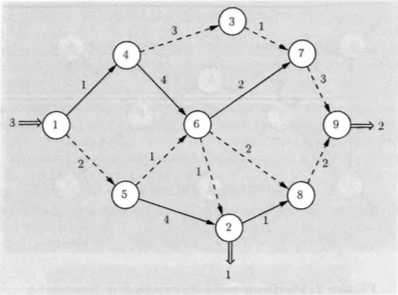
\includegraphics[width=0.5\textwidth]{hw5_exercise7.10.png}
    \end{center}
    \begin{parts}
        \part \textit{What are the values of the arc flows corresponding to this basic solution? Is this a basic feasible solution?}
        \newline See the arc flows below for $f_T$, the remaining flows are 0. Yes, this basic solution is feasible (and hence a BFS) since no flows violate the arc directions. 
        \begin{align*}
            T &= \left\{\begin{matrix}
                (1,5), (5,6), (6,2), (6,8), (8,9), (7,9), (3,7), (4,3)
            \end{matrix}\right\}\\
            A\setminus T &= \left\{\begin{matrix}
                (1,4), (4,6), (6,7), (5,2), (2,8)
            \end{matrix}\right\}
        \end{align*}
        \begin{align*}
            f_T^\top = \begin{array}{cccccccc}
                (1,5) & (5,6) & (6,2) & (6,8) & (8,9) & (7,9) & (3,7) & (4,3)\\\hline
                3 & 3 & 1 & 2 & 2 & 0 & 0 & 0
            \end{array}
        \end{align*}

        \part \textit{For this basic solution, find the reduced cost of each arc in the network}
        \begin{align*}
            c_T &= \begin{array}{|cccccccc|}
                (1,5) & (5,6) & (6,2) & (6,8) & (8,9) & (7,9) & (3,7) & (4,3)\\\hline
                2 & 1 & 1 & 2 & 2 & 3 & 1 & 3 
            \end{array}\\
            c_{A\setminus T} &= \begin{array}{|ccccc|}
                (1,4) & (4,6) & (6,7) & (5,2) & (2,8)\\\hline
                1 & 4 & 2 & 4 & 1                
            \end{array}
        \end{align*}
        \newline Since $T$ forms a basis for a basic feasible solution, the reduced cost of all arcs in $T$ are 0 by construction. Suffice to determine reduced costs of arcs in $A\setminus T$.
        \begin{align*}
            p^\top = \begin{array}{|ccccccccc|}
                p_1 & p_2 & p_3 & p_4 & p_5 & p_6=0 & p_7 & p_8 & p_9\\\hline
                3 & -1 & 0 & 3 & 1 & 0 & -1 & -2 & -4               
            \end{array}
        \end{align*}
        \begin{align*}
            \bar c_T &= \begin{array}{|cccccccc|}
                (1,5) & (5,6) & (6,2) & (6,8) & (8,9) & (7,9) & (3,7) & (4,3)\\\hline
                0&0&0&0&0&0&0&0
            \end{array}\\
            \bar c_{A\setminus T} &= \begin{array}{|ccccc|}
                (1,4) & (4,6) & (6,7) & (5,2) & (2,8)\\\hline
                1 - (3 - 3) & 4 - (3 - 0) & 2 - (0 + 1) & 4 - (1 + 1) & 1 - (-1 + 2)\\
                1 & 1 & 1 & 2 & 0                
            \end{array}
        \end{align*}

        \part \textit{Is this basic solution optimal?}
        \newline Yes, the reduced cost vector is all nonnegative, indicating that we have reached a minimal-cost flow pattern

        \part \textit{Does there exist a nondegenerate optimal basic feasible solution?}
        \newline No there does not. Since we are at an optimal solution, by complementary slackness we know
        \begin{align*}
            (c_{i,j} - (p_i - p_j))f_{i,j} = 0 \;\forall\;(i,j)\in A
        \end{align*}
        We have just calculated the set of $(i,j)$ for which $\bar c_{i,j} = c_{i,j} - (p_i - p_j) = 0$. Call this set $\mathcal Z$ and note $\mathcal Z = T\cup\{(2,8)\}$. It's over this set that flows may be nonzero to be feasible and preserve optimality.

        We also note by the nature of this graph that we must have zero-flows on $f_{4,3}, f_{3,7}, f_{7,9}$. Reasoning: there is 0 flow into node $4$ and the only flow over line $(4,3)$ is from node $4$. We use the same logic for lines $(3,7), (7,9)$. Note that these three arcs, $(4,3), (3,7), (7,9) \in \mathcal Z$.
        
        Since $|\mathcal Z| = 9$ and the zero-flow constraints requires 3 of the lines in $\mathcal Z$ to have zero flows, we are left with $9-3=6$ possible lines with nonzero flow for any optimal solution. Since optimal solutions are all tree solutions, nondegenerate solutions must have $n-1=8$ arcs with nonzero flows. Therefore all optimal solutions for this graph are degenerate (since $8 > 6$).
        
        
        \part \textit{Find an optimal dual solution}
        In step (B) we calculated vector $p$. Since we have shown that flow vector $f$ corresponding to spanning tree $T$ is an optimal solution, by strong duality we know $p$ is an optimal dual solution
        \begin{align*}
            p^\top = \begin{array}{|ccccccccc|}
                p_1 & p_2 & p_3 & p_4 & p_5 & p_6=0 & p_7 & p_8 & p_9\\\hline
                3 & -1 & 0 & 3 & 1 & 0 & -1 & -2 & -4               
            \end{array}
        \end{align*}
        Note since the columns of A defining the graph are linearly dependent, we can have more than one such optimal dual solution.
        
        
        \part \textit{By how much can we increase $c_{56}$ [the cost of arc (5,6)] and still have the same optimal basic feasible solution?}
        \newline Let $c_{56} = 1 + \gamma$ and we'll solve for $\gamma$. Returning to our reduced cost vectors
        {\small
        \begin{align*}
            p^\top &= \begin{array}{|ccccccccc|}
                p_1 & p_2 & p_3 & p_4 & p_5 & p_6=0 & p_7 & p_8 & p_9\\\hline
                3 + \gamma & -1 & 0 & 3 & 1 + \gamma & 0 & -1 & -2 & -4               
            \end{array}\\
            \bar c_T &= \begin{array}{|cccccccc|}
                (1,5) & (5,6) & (6,2) & (6,8) & (8,9) & (7,9) & (3,7) & (4,3)\\\hline
                2 - (3 + \gamma - 1 - \gamma) & 1+\gamma - (1 + \gamma - 0) & 0 & 0 & 0  & 0 & 0 & 0 \\
                0&0& 0 & 0 & 0  & 0 & 0 & 0
            \end{array}\\
            \bar c_{A\setminus T} &= \begin{array}{|ccccc|}
                (1,4) & (4,6) & (6,7) & (5,2) & (2,8)\\\hline
                1 - (3+\gamma - 3) & 4 - (3 - 0) & 2 - (0 + 1) & 4 - (1+\gamma + 1) & 1 - (-1 + 2)\\
                1-\gamma & 1 & 1 & 2-\gamma & 0                
            \end{array}
        \end{align*}
        }
        In order for our reduced costs to remain nonnegative, $\gamma \leq 1$. 
        
        
        \part \textit{If we increase the supply at node 1 and the demand at node 9 by a small positive amount $\delta$, what is the change in the value of the optimal cost?}
        \newline In the optimal solution, which by definition is a tree soltuion, the cost of the path from node 1 to node 9 is
        \begin{align*}
            c_{T_{path(1,9)}}^\top = \begin{array}{|cccc|}
                (1,5) & (5,6) & (6,8) & (8,9)\\\hline
                2 & 1 & 2 & 2
            \end{array}
        \end{align*}
        And increasing supply at node 1 and demand at node 9 by $\delta$, only the flows over this path from node 1 to node 9 are affected. Flows become
        \begin{align*}
            f_{T_{path(1,9)}}^\top = \begin{array}{|cccc|}
                (1,5) & (5,6) & (6,8) & (8,2)\\\hline
                3 + \delta & 3 + \delta & 2 + \delta & 2 + \delta
            \end{array}
        \end{align*}
        The change in the value of the optimal cost is just the change in flow, $\delta$, times the cost of the path this change follows:
        \begin{align*}
           \Delta \text{cost} = \delta \sum_{(i,j)\in T_{path(1,9)}}c_{i,j} = \delta \times (2 + 1 + 2 + 2) = 7\delta
        \end{align*}
        
        
        \part \textit{Does this problem have a special structure that makes it simpler than the general uncapacitated network flow problem?}
        \newline We make a few observations about this graph structure that makes it simpler than a general network flow problem
        \begin{enumerate} 
            \item \textbf{Integer solutions:} This graph has integer costs and integer injections/withdrawals. From BT Theorem 7.5 and Corrolary 7.2, every basic solution has integer coordinates and there exists an integer optimal flow vector. Also, this theorem/corrolary states that every dual basic solution has integer coordinates and there exists an integer optimal solution to the dual problem.
            \item \textbf{Shortest path algorithms:} This graph is a single-source, multi-sink min-cost flow. It is on a network without capacities. Because of this, the optimal flow is the sum of two shortest-path flows from the source to each sink. No arc capacity means that these problems aren't coupled. The textbook shows that there are even more efficient algorithms for solving shortest-path problems
        \end{enumerate}
    \end{parts}




    % ============ QUESTION 8.5 ==============
    \question \textbf{Exercise 8.5 (Characterization of full-dimensional polyhedra):} 
    \newline\textbf{(Given)} Polyhedron $P =\{x \in \mathbb R^n \mid Ax \geq b\}$ is bounded and all rows of $A$ are nonzero. 
    \newline\textbf{(Show)} The following are equivalent
    \begin{enumerate}
        \item The polyhedron $P$ has full dimension (has positive volume)
        \item $\exists\; x \in P$ such that $Ax > b$
        \item There are $n + 1$ extreme points of $P$ that do not lie on a common hyperplane
    \end{enumerate}
    \begin{parts}
        \part ($1 \Longrightarrow 3$): \textbf{(Contrapositive, $\neg 3 \Longrightarrow \neg 1$)} Suppose any $n+1$ extreme points of $P$ lie on a common hyperplane. This implies that \emph{all} extreme points of $P$ lie on a common hyperplane. 

        To see this, pick any extreme point $x^0$ and choose any $n$ additional extreme points $x^1,\dots,x^n$ (WLOG, assume at least $n$ exist). By assumption, the set $\{x^0,\dots,x^n\}$ lies on some hyperplane
        \begin{align*}
            H = \{x\mid c^\top x = \beta\}
        \end{align*}
        Now consider any other extreme point $y$. The set $\{y, x^1,\dots,x^n\}$ also contains $n+1$ extreme points, so by assumption it lies on 
        some hyperplane 
        \begin{align*}
            H_y = \{x \mid c_y^\top x = \beta_y\}
        \end{align*}
        Since the $n$ points $x^1,\dots,x^n$ lie on both $H$ and $H_y$, and $n$ affinely independent points determine a unique hyperplane, we must have $H_y = H$ and all extreme points of $P$ lie on the same hyperplane.
        
        Now consider the convex hull of all extreme points, 
        \begin{align*}
            P_S = \{y \mid y = \sum_{i=1}^k \lambda_i x^i, \sum_{i=1}^k \lambda_i = 1\} \text{ for $x^i$ the extreme points of $P$}
        \end{align*}
        Since all extreme points lie on a common hyperplane in $\mathbb R^n$, $\dim(P_S) = n-1$. And since any bounded polyhedron is equivalent to the convex hull of its extreme points, $\dim(P) = \dim(P_S) = n-1$. Therefore, $P$ is not full dimension. 

        \part ($3 \Longrightarrow 2$): Consider arbitrary constraint of $P$, $a_i^\top x \geq b_i$. Existence of $n+1$ extreme points of $P$ not on a common hyperplane implies that there exists at least one extreme point, $x^{(i)}$, for which $a_i^\top x^{(i)} > b_i$ (since if all sets of $n+1$ extreme points satisfied $a_i^\top x = b_i$, they would all lie on this same hyperplane and violate our assumption). 
        
        Now for each constraint, $j$, we may choose extreme point $x^{(j)}$ for which the constraint is not binding and form a convex combination of all such points:
        \begin{align*}
            \tilde x = \sum_{i=1}^m \lambda_i x^{(i)},\; \sum_{i=1}^m \lambda_i = 1,\;\lambda_i > 0
        \end{align*}
        This new point, $\tilde x$, is feasible since convex combinations of feasible points remain feasible, and it lies on the interior of $P$ ($A\tilde x > b$) because at least one term in the sum is strictly greater than $b_i\;\forall i\in[m]$:
        \begin{align*}
            a_i^\top \tilde x = \sum_{j=1}^m \lambda_j a_i^\top x^{(j)} > \sum_{j=1}^m \lambda_jb_i = b_i
            \; \sum_{i=1}^m \lambda_i = 1,\; \lambda_i > 0
        \end{align*}
        Therefore, $P$ contains a strictly feasible point.

        \part ($2 \Longrightarrow 1$): Consider such point $x_0 \in P$ such that $Ax_0 > b$. Since $x_0$ is in the interior of $P$, define for each inequality, $i$, its signed distance from $x_0$ to that hyperplane
        \begin{align*}
            d_i = \frac{a_i^\top x_0 - b_i}{||a_i||_2} > 0
        \end{align*}
        The smallest such distance, $\epsilon$, to any hyperplane $i$ is $\epsilon=\min_i d_i$. Note $\epsilon > 0$ since all $d_i > 0\;\forall\;i \in [m]$. 
        Now consider Euclidean ball $B(x_0, \epsilon) = \{y \mid (y - x_0)^\top(y-x_0) \leq \epsilon\}$. Note that $B(x_0, \epsilon)$ has full dimension (since $\epsilon > 0$). Lastly, $B(x_0, \epsilon)\subseteq P$ by construction of maximum ball contained in $P$. These two conditions imply that $P$ has full dimension.
    \end{parts}
\end{questions}
\end{document}